\section{Ausführungspläne}
\label{plan}

Gegeben seien folgende Relationen:

\texttt{Employee (\underline{num}, fname, lname, addr, mgr[employee], \beamertxt{\\}dep[department])}

\texttt{Department (\underline{num}, name, mgr[employee])}

\texttt{Project (\underline{num}, dep[department], mgr[employee])}

\texttt{Works\_on (\underline{proj[project], empl[employee]})}

Setzen Sie folgende SQL-Anweisungen in nicht-optimierte Operatorgraphen um. Verwenden Sie dafür die Baum-Notation von Vorlesungsfolie~\Operatorgraph. % stimmt noch (KMW, 04.12.2018)

\fbox{\begin{minipage}{\textwidth}
\paragraph{Hinweis:} Zur weiteren Übung können Sie das Tool DBSnap verwenden: \\
	\DBSnap \\
	Bitte beachten: Es führt bei der Projektion zusätzlich eine Duplikateliminierung durch.\\
	Zum Testen eigener Anfragen können Sie auch gerne das Webinterface von Umbra verwenden : \\
	\Umbra

	\begin{note}
		Literatur: Y. N. Silva et al.: DBSnap: Learning Database Queries by Snapping Blocks, SIGCSE 2015, DOI \url{http://dx.doi.org/10.1145/2676723.2677220}
	\end{note}
\end{minipage}}
\begin{enumerate}[a)]

	\item Alle MitarbeiterInnen und ihre Vorgesetzten.
	\begin{lstlisting}
SELECT e.fname, e.lname, s.fname, s.lname
FROM   employee e, employee s
WHERE  e.mgr = s.num
	\end{lstlisting}

\cprotEnv
	\begin{solution}
	\begin{tikzpicture}
		\node (proj) at(0, 0) {\texttt{PROJ(\hspace{0.5cm} , (e.fname, e.lname, s.fname, s.lname))} };
		\node (sel) [below of =proj, xshift=-1.2cm] {\texttt{SEL(\hspace{0.5cm} , (e.mgr = s.num))} };
		\node (cross)[below of =sel] {\texttt{CROSS(\qquad, \qquad)} };
		\node (rename1) [below of = cross, xshift=-0.5cm] {\texttt{RENAME(\qquad, e)}};
		\node (rename2) [below of =cross, xshift=3.5cm] {\texttt{RENAME(\qquad, s)}};
		\node (emp1) [below of = rename1, xshift=0.3cm] {\texttt{employee}};
		\node (emp2) [below of =rename2, xshift=0.3cm] {\texttt{employee}};

		\draw[-triangle 60] ($(sel.north west)+(0.5,0)$) -- ($(proj.south) + (-3.4,0)$);
		\draw[-triangle 60] ($(cross.north) +(-1.2,0)$) -- ($(sel.south) + (-1.2,0)$);
		\draw[-triangle 60] ($(rename1.north) + (-0.9,0)$) -- ($(cross.south) + (0.0,0.1)$);
		\draw[-triangle 60] ($(rename2.north) + (-1.2,0)$) -- ($(cross.south) + (0.8,0.1)$);
		\draw[-triangle 60] (emp1) -- ($(rename1.south) + (0.3,0.1)$);
		\draw[-triangle 60] (emp2) -- ($(rename2.south) + (0.3,0.1)$);
	\end{tikzpicture}
\paragraph{\color{solutioncolor}Anmerkung:} Die folgenden Darstellungen sind äquivalent nutzbar:\\
\begin{minipage}{0.49\textwidth}
\begin{lstlisting}
- PROJ( , (e.fname, e.lname,
           s.fname, s.lname))
  - SEL( , (e.mgr = s.num))
    - CROSS( , )
      - RENAME( , e)
        - employee
      - RENAME( , s)
        - employee
\end{lstlisting}
\end{minipage}
\begin{minipage}{0.49\textwidth}
	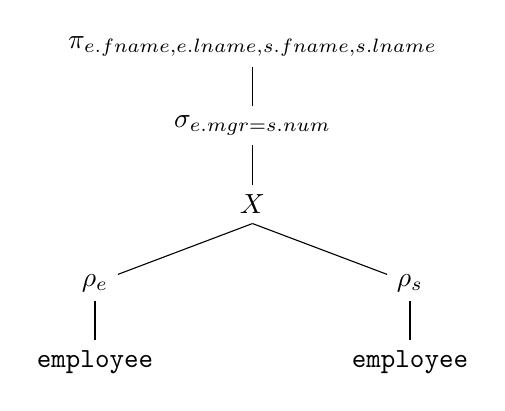
\begin{tikzpicture}
	\node (proj) at(0, 0) {$\pi_{e.fname, e.lname, s.fname, s.lname}$};
	\node (sel) [below of =proj] {$\sigma_{e.mgr = s.num}$};
	\node (cross)[below of =sel] {$X$};
	\node (rename1) [below of = cross, xshift=-2cm] {$\rho_{\text{e}}$};
	\node (rename2) [below of =cross, xshift=2cm] {$\rho_{\text{s}}$};
	\node (emp1) [below of = rename1] {\texttt{employee}};
	\node (emp2) [below of =rename2] {\texttt{employee}};
	
	\draw (sel) -- (proj.south);
	\draw (cross) -- (sel.south);
	\draw (rename1) -- (cross.south);
	\draw (rename2) -- (cross.south);
	\draw (emp1) -- (rename1.south);
	\draw (emp2) -- (rename2.south);
\end{tikzpicture}

\begin{note}
	Anmerkung: Diese Darstellung könnte vor allem für Lehramtsstudierende wichtig sein,
	da sie prinzipiell im Staatsexamen erwartet werden kann.
\end{note}
\end{minipage}
Oder auch nicht als Baum strukturiert:
\[\pi_{e.fname, e.lname, s.fname, s.lname}(\sigma_{e.mgr = s.num}(X(\rho_{\text{e}}(employee), \rho_{\text{s}}(employee))))\]
	\end{solution}

\beamertxt{\pagebreak}

	\item Alle MitarbeiterInnen der Forschungsabteilung.
	\begin{lstlisting}
SELECT e.fname, e.lname, e.addr
FROM   employee e
JOIN   department d
ON     d.num = e.dep
WHERE  d.name = 'Research';
	\end{lstlisting}

	\begin{solution}
	\begin{tikzpicture}
		\node (proj) at (0, 0) {\texttt{PROJ(\qquad , (e.fname, e.lname, e.addr))} };
		\node (sel)[below of =proj, xshift=0.5cm] {\texttt{SEL(\qquad , (d.name = 'Research'))} };

		\node (join)[below of =sel, xshift=1cm] {\texttt{JOIN(\qquad, \qquad, (d.num = e.dep))} };
		\node (renamed)[below of =join, xshift = 2cm] {\texttt{RENAME(\qquad, d)}};
		\node (renamee)[below of =join, xshift =-3cm] {\texttt{RENAME(\qquad, e)}};
		\node (dept)[below of =renamed, xshift=0.3cm] {\texttt{department} };
		\node (emp)[below of =renamee, xshift=0.3cm] {\texttt{employee} };

		\draw[-triangle 60] (dept) -- ($(renamed.south) + (0.3,0.1)$);
		\draw[-triangle 60] (emp) -- ($(renamee.south) + (0.3,0.1)$);
		\draw[-triangle 60] (renamed) -- ($(join.south) + (-0.9,0.1)$);
		\draw[-triangle 60] ($(renamee.north) + (-0.8, 0)$) -- ($(join.south) + (-2,0.1)$);
		\draw[-triangle 60] ($(join.north west) + (0.6, 0)$) -- ($(sel.south) + (-1.9,0.1)$);
		\draw[-triangle 60] ($(sel.north west) + (0.6, 0)$) -- ($(proj.south) + (-2.3,0.1)$);
	\end{tikzpicture}
	\end{solution}

  \item Alle Abteilungen mit mehr als 10 Mitarbeitern.
	\begin{lstlisting}
SELECT   d.name
FROM     employee e
JOIN     department d
ON       d.num = e.dep
GROUP BY d.num, d.name
HAVING   count(d.num) > 10
	\end{lstlisting}

	\begin{solution}
	\begin{tikzpicture}
		\node (proj) at (0, 0) {\texttt{PROJ(\qquad , (d.name))} };
		\node (hav)[below of =proj, xshift=2cm] {\texttt{SEL(\qquad , (aggregierte $>$ 10))} };

		\node (group)[below of =hav, xshift=3.7cm] {\texttt{GROUP(\qquad , (d.num, d.name), ((count(d.num), aggregierte)))}};
		\node (join)[below of =group, xshift=-1.5cm] {\texttt{JOIN(\qquad, \qquad, (d.num = e.dep))} };
		\node (renamed)[below of =join, xshift = 1.5cm] {\texttt{RENAME(\qquad, d)} };
		\node (renamee)[below of =join, xshift =-2.5cm] {\texttt{RENAME(\qquad, e)} };
		\node (dept)[below of =renamed, xshift=0.3cm] {\texttt{department} };
		\node (emp)[below of =renamee, xshift=0.3cm] {\texttt{employee} };

		\draw[-triangle 60] ($(renamed.north west) + (0.8,0)$) -- ($(join.south) + (-0.8,0.1)$);
		\draw[-triangle 60] ($(renamee.north west) + (0.8,0)$) -- ($(join.south) + (-1.9,0.1)$);
		\draw[-triangle 60] (dept) -- ($(renamed.south) + (0.3,0.1)$);
		\draw[-triangle 60] (emp) -- ($(renamee.south) + (0.3,0.1)$);
		\draw[-triangle 60] ($(join.north west) + (0.7,0)$) -- ($(group.south) + (-4.3,0.1)$);
		\draw[-triangle 60] ($(group.north west) + (0.8,0)$)-- ($(hav.south) + (-1.5,0.1)$);
		\draw[-triangle 60] ($(hav.north west) + (0.5, 0)$) -- ($(proj.south) + (-0.6,0.1)$);
	\end{tikzpicture}
	\end{solution}

	\item Alle MitarbeiterInnen mit Nachnamen Smith, die eine operative Abteilung leiten oder einem Projekt zugeordnet sind.
	\nt{Diese Aufgabe + Optimierung evtl bis zum Ende schieben und nur machen wenn noch Zeit ist / bei der der Durchführung abbrechen und auf ML verweisen.}
	\begin{lstlisting}
SELECT e.lname
FROM ((SELECT p.num, e.lname
    FROM   project p, department d, employee e
    WHERE  d.num = p.dep
    AND    d.mgr = e.num
  )
  UNION
  ( SELECT p.num, e.lname
    FROM   project p, works_on w, employee e
    WHERE  p.num = proj
    AND    e.num = empl
  )
)
WHERE e.lname = 'Smith';
	\end{lstlisting}

	\begin{solution}
	\begin{tikzpicture}
		\node (proj_top) at(0, 0) {\small{\texttt{PROJ(\hspace{0.5cm}, (e.lname))} } };
		\node (sel_top) [below of =proj_top, xshift=1.7cm] {\small{\texttt{SEL(\hspace{0.5cm}, (e.lname = 'Smith'))} } };
		\node (union) [below of =sel_top, xshift=-0.5cm] {\small{\texttt{UNION(\qquad, \qquad)} } };

		\node (proj_left) [below of =union, xshift = 6.2cm] {\small{\texttt{PROJ(\hspace{0.5cm}, (p.num, e.lname))} } };
		\node (proj_right) [below of =union, xshift = -1.7cm] {\small{\texttt{PROJ(\hspace{0.5cm}, (p.num, e.lname))} } };

		\node (sel_left) [below of =proj_left, xshift=0.5cm] {\small{\texttt{SEL(\hspace{0.5cm}, (d.num = p.dep} } };
		\node (sel_left2) [below of =sel_left, xshift =1cm, yshift = 0.6cm] {\small{\texttt{AND d.mgr = e.num))} } };
		\node (sel_right) [below of =proj_right, xshift =0.9cm] {\small{\texttt{SEL(\hspace{0.5cm}, (p.num = w.proj AND} } };
		\node (sel_right2) [below of =sel_right, xshift =0.7cm, yshift = 0.6cm] {\small{\texttt{e.num = w.empl))} } };

		\node (cross_left) [below of =sel_left, xshift =0.5cm, yshift =-0.5cm] {\small{\texttt{CROSS(\qquad, \qquad, \qquad)} } };
		\node (cross_right) [below of =sel_right, xshift =0cm, yshift =-0.5cm] {\small{\texttt{CROSS(\qquad, \qquad, \qquad)} } };

		\node (rename_emp_left) [below of =cross_left, xshift =-2cm] {\texttt{RENAME(\qquad, e)}};
		\node (rename_dept_left) [below of =cross_left, xshift =0.5cm, yshift =-0.5cm] {\texttt{RENAME(\qquad, d)} };
		\node (rename_project_left) [below of =cross_left, xshift =2cm] {\texttt{RENAME(\qquad, p)}};
		\node (rename_emp_right) [below of =cross_right, xshift =-1.5cm] {\texttt{RENAME(\qquad, e)}};
		\node (rename_works_right) [below of =cross_right, xshift =1cm, yshift =-0.5cm] {\texttt{RENAME(\qquad, w)}};
		\node (rename_project_right) [below of =cross_right, xshift =2.3cm] {\texttt{RENAME(\qquad, p)}};

		\node (emp_left) [below of =rename_emp_left, xshift=0.3cm] {\texttt{employee} };
		\node (dept_left) [below of =rename_dept_left, xshift=0.3cm] {\texttt{department}};
		\node (project_left) [below of =rename_project_left, xshift=0.3cm] {\texttt{project} };
		\node (emp_right) [below of =rename_emp_right, xshift=0.3cm] {\texttt{employee} };
		\node (works_right) [below of =rename_works_right, xshift=0.3cm] {\texttt{works\_on} };
		\node (project_right) [below of =rename_project_right, xshift=0.3cm] {\texttt{project} };

		\draw[-triangle 60] ($(sel_top.north west) + (0.4, 0)$) -- ($(proj_top.south) + (-0.8,0.1)$);
		\draw[-triangle 60] ($(union.north west) + (0.6, 0)$) -- ($(sel_top.south) + (-1.6,0.1)$);

		\draw[-triangle 60] ($(proj_left.north west) + (0.4, 0)$) -- ($(union.south) + (0.8, 0.1)$);
		\draw[-triangle 60] ($(proj_right.north west) + (0.6, 0)$) -- ($(union.south) + (-0.2, 0.1)$);

		\draw[-triangle 60] ($(sel_left.north west) + (0.4, 0)$) -- ($(proj_left.south) + (-1.35,0.1)$);
		\draw[-triangle 60] ($(sel_right.north west) + (0.4, 0)$) -- ($(proj_right.south) + (-1.35,0.1)$);

		\draw[-triangle 60] ($(cross_left.north west) + (0.7, 0 )$) -- ($(sel_left.south) + (-1.1,0.1)$);
		\draw[-triangle 60] ($(cross_right.north west) + (0.7, 0 )$) -- ($(sel_right.south) + (-1.6,0.1)$);

		\draw[-triangle 60] ($(rename_emp_left.north west) + (0.8, 0)$) -- ($(cross_left.south) + (-0.65,0.1)$);
		\draw[-triangle 60] ($(rename_dept_left.north west) + (0.8, 0)$) -- ($(cross_left.south) + (0.4,0.1)$);
		\draw[-triangle 60] ($(rename_project_left.north west) + (0.8, 0)$) -- ($(cross_left.south) + (1.4,0.1)$);
		\draw[-triangle 60] ($(rename_emp_right.north west) + (0.8, 0)$) -- ($(cross_right.south) + (-0.65,0.1)$);
		\draw[-triangle 60] ($(rename_works_right.north west) + (0.8, 0)$) -- ($(cross_right.south) + (0.4,0.1)$);
		\draw[-triangle 60] ($(rename_project_right.north west) + (0.8, 0)$) -- ($(cross_right.south) + (1.4,0.1)$);

		\draw[-triangle 60] (emp_left) -- ($(rename_emp_left.south) + (0.3,0.1)$);
		\draw[-triangle 60] (dept_left) -- ($(rename_dept_left.south) + (0.3,0.1)$);
		\draw[-triangle 60] (project_left) -- ($(rename_project_left.south) + (0.3,0.1)$);
		\draw[-triangle 60] (emp_right) -- ($(rename_emp_right.south) + (0.3,0.1)$);
		\draw[-triangle 60] (works_right) -- ($(rename_works_right.south) + (0.3,0.1)$);
		\draw[-triangle 60] (project_right) -- ($(rename_project_right.south) + (0.3,0.1)$);
	\end{tikzpicture}
	\end{solution}

\end{enumerate}
